% FONTE TEMA https://github.com/matze/mtheme
\documentclass[aspectratio=1610]{beamer}
%\documentclass[aspectratio=1610, handout]{beamer}
\usepackage[utf8]{inputenc}
\usepackage{ragged2e}
\usepackage{xcolor}
\usepackage[italian]{babel}
\usepackage{multirow}
\usepackage{silence}
\WarningFilter{beamer}{}
\WarningFilter{metropolis}{}
\usetheme[progressbar=frametitle,titleformat=smallcaps]{metropolis}
\setbeamertemplate{frame numbering}[fraction]
\setbeamercovered{dynamic}
\definecolor{rosso}{RGB}{255, 0, 0}
\definecolor{giallo}{RGB}{254,212,23}
\hypersetup{colorlinks=true,linkcolor=black,urlcolor=rosso}
\setbeamercolor{palette primary}{fg=black, bg=giallo}
\setbeamercolor{background canvas}{bg=white}
\setbeamercolor{normal text}{fg=black}
\setbeamercolor{progress bar}{fg=rosso}
\setbeamercolor{framesubtitle}{fg=rosso}
\setbeamercolor{normal text .dimmed}{fg=giallo}
\setbeamercolor{block title alerted}{fg=rosso, bg=giallo}
\setbeamerfont{caption}{size=\tiny}
\setbeamerfont{caption name}{size=\tiny}
\setlength{\abovecaptionskip}{0pt}
\makeatletter
\metroset{block=fill}
\setlength{\metropolis@progressinheadfoot@linewidth}{1pt} 
\setlength{\metropolis@progressonsectionpage@linewidth}{1pt}
\setlength{\metropolis@titleseparator@linewidth}{1pt}
\makeatother

\title{SISTEMA ESACDECIMALE}
\subtitle{Conversioni tra sistemi di numerazione}
\date{}
\institute{}

\begin{document}

\begin{frame}[plain, noframenumbering]
    \titlepage
\end{frame}

\begin{frame}{SISTEMA NUMERICO POSIZIONALE IN BASE 16}
    \begin{alertblock}{DEFINIZIONE}
        \begin{minipage}{0.98\linewidth}
            \justifying
            Il sistema numerico esadecimale è molto utilizzato in ambito informatico, in quanto 
            più la base di un sistema di numerazione è maggiore, meno sarà lunga la rappresentazione 
            della quantità rappresentata.\\ 
            \pause
            Essendo la rappresentazione dei dati all'interno di un elaboratore sempre in codifica 
            binaria (base 2), è comodo compattarne la rappresentazione utilizzando le proprietà 
            di conversione tra binario e esadecimale.\\
            \bigskip
            \textbf{SIMBOLI DEL SISTEMA NUMERICO POSIZIONALE ESADECIMALE}\\
            \bigskip
            \only<3->{
                \begin{tabular}{r|c|c|c|c|c|c|c|c|c|c|c|c|c|c|c|c}
                    \textbf{HEX} & 0 & 1 & 2 & 3 & 4 & 5 & 6 & 7 & 8 & 9 & \textbf{\large{A}} & \textbf{\large{B}} & \textbf{\large{C}} & \textbf{\large{D}} & \textbf{\large{E}} & \textbf{\large{F}} \\
                    \textbf{DECIMALE} & 0 & 1 & 2 & 3 & 4 & 5 & 6 & 7 & 8 & 9 & 10 & 11 & 12 & 13 & 14 & 15 \\
                \end{tabular}
            }
        \end{minipage}
    \end{alertblock}
\end{frame}

\begin{frame}{ESEMPIO DI CODIFICA HEX}
    \begin{columns}
        \column{.5\textwidth}
            \begin{tabular}{c|c|c}
                \textbf{COLORE} & \textbf{ESADECIMALE} & \textbf{DECIMALE} \\
                \hline
                \hline
                \textcolor{red}{RED} & \#\textcolor{red}{FF}0000 & \textcolor{red}{255}, 0, 0 \\
                \hline
                \textcolor{green}{GREEN} & \#00\textcolor{green}{FF}00 & 0, \textcolor{green}{255}, 0 \\
                \hline
                \textcolor{blue}{BLUE} & \#0000\textcolor{blue}{FF} & 0, 0, \textcolor{blue}{255} \\
                \hline
                YELLOW & \#FFFF00 & 255, 255, 0 \\
            \end{tabular}\\
            \bigskip
            \tiny{\textbf{Tools}}\\
            \tiny{\href{https://www.canva.com/colors/color-wheel/}{Ruota dei colori}}\\
            \tiny{\href{https://www.w3schools.com/colors/colors_rgb.asp}{RGBA}}\\
        \column{.5\textwidth}
            \begin{figure}
                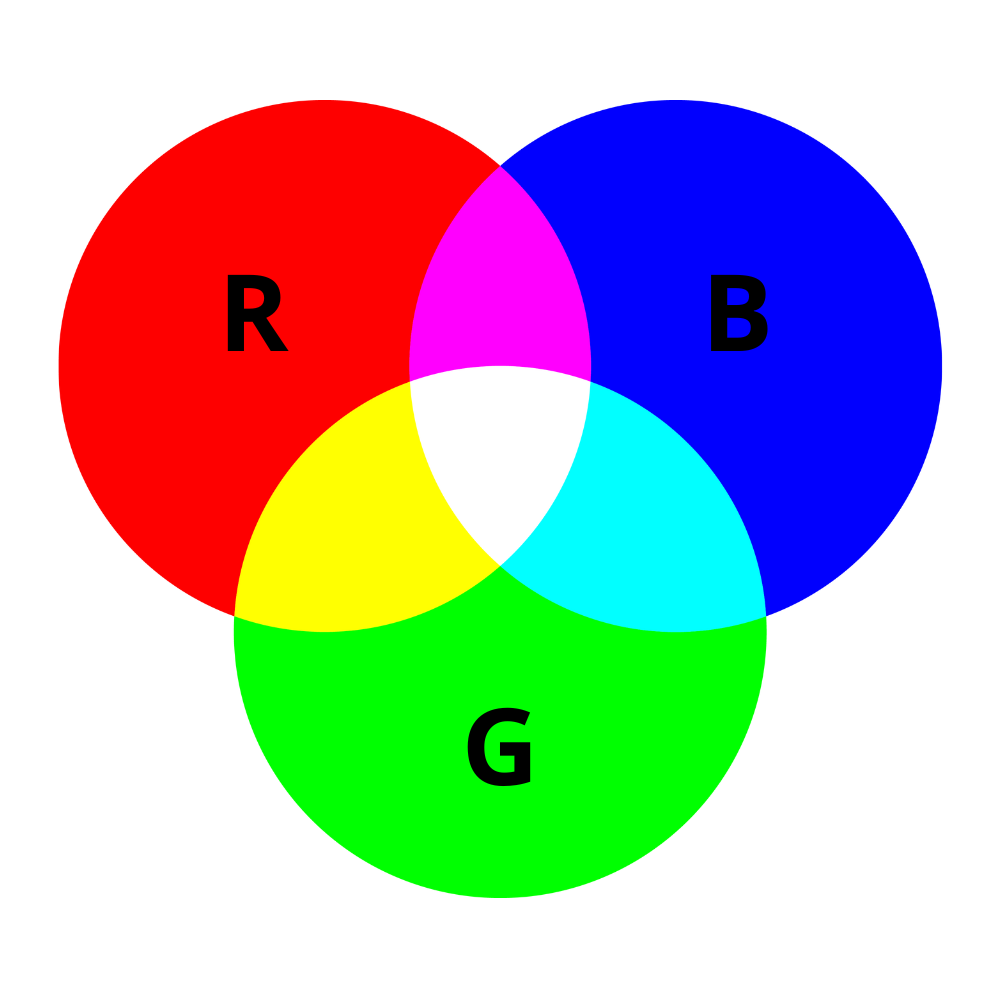
\includegraphics[width=\linewidth]{img/rgb.png}
                \caption{{creata con \href{www.canva.com}{Canva}}}
            \end{figure}
    \end{columns}
\end{frame}

\section{CONVERSIONE DA ESADECIMALE A DECIMALE}

\begin{frame}{CONVERSIONE ESADECIMALE - DECIMALE}
    \centering
    \huge
    $(3A6C)_{16}$
\end{frame}

\begin{frame}{CONVERSIONE ESADECIMALE - DECIMALE}
\centering
    \begin{tabular}{r||c|c|c|c}
        \textbf{NUMERO ESADECIMALE} & 3 & \textbf{A} & 6 & \textbf{C} \\
        \hline
        \pause
        \textbf{VALORE DECIMALE} & 3 & 10 & 6 & 12 \\
        \hline
        \pause
         & x & x & x & x \\
        \hline
         \textbf{PESI} & $16^3$ & $16^2$ & $16^1$ & $16^0$ \\
        \hline
         & = & = & = & = \\
        \hline
        \pause
        \textbf{PARZIALI} & 12288 & 2560 & 96 & 12 \\
        \\
        \hline
        \pause
        \textbf{QUANTIT\'A (DECIMALE)} & \multicolumn{4}{c}{$\mathbf{12288 + 2560 + 96 + 12 = 14956}$} \\
    \end{tabular}
    \pause
    \begin{alertblock}{COVERSIONE BINARIO - DECIMALE}
        \begin{minipage}{0.98\linewidth}
            \centering
            \huge
            $(3A6C)_{16} = (14956)_{10}$
        \end{minipage}
    \end{alertblock}
\end{frame}

\section{CONVERSIONE DA DECIMALE A ESADECIMALE}

\begin{frame}{CONVERSIONE ESADECIMALE - DECIMALE}
    \centering
    \huge
    $(14956)_{10}$
\end{frame}

\begin{frame}{COVERSIONE DECIMALE - ESADECIMALE}
    \centering
    \begin{tabular}{r||c|c|c}
        \textbf{NUMERO DECIMALE} & 14956 & \textbf{RESTO} & \textbf{ESADECIMALE} \\
        \hline
        \pause
        14956 : \textbf{16} = & 934 & \textbf{12} & \textbf{C}\\
        \hline
        \pause
        934 : \textbf{16} = & 58 & 6 & 6 \\
        \hline
        \pause
        58 : \textbf{16} = & 3 & \textbf{10} & \textbf{A} \\
        \hline
        \pause
        3 : \textbf{16} = & \textcolor{red}{\textbf{0}} & 3 & 3 \\
    \end{tabular}
    \pause
    \begin{minipage}{0.25\linewidth}
        \begin{tikzpicture}[remember picture,overlay]
            \draw[->, ultra thick, rosso] (8,0) -- (8,2.3) node[above] {};
        \end{tikzpicture}
    \end{minipage}
    \begin{alertblock}{COVERSIONE DECIMALE - ESADECIMALE}
        \begin{minipage}{0.98\linewidth}
            \centering
            \huge
            $(14956)_{10} = (3A6C)_{16}$
        \end{minipage}
    \end{alertblock}
\end{frame}

\section{CONVERSIONE DA ESADECIMALE A BINARIO}

\begin{frame}{CONVERSIONE ESADECIMALE - BINARIO}
    \centering
    \huge
    $(3A6C)_{16}$
\end{frame}

\begin{frame}{COVERSIONE ESADECIMALE - BINARIO}
    \centering
    \begin{tabular}{r||c|c|c|c}
        \textbf{NUMERO ESADECIMALE} & 3 & \textbf{A} & 6 & \textbf{C} \\
        \hline
        \pause
        \textbf{VALORE DECIMALE} & 3 & \textbf{10} & 6 & \textbf{12} \\
        \hline
        \pause
        \textbf{NUMERO BINARIO} & 11 & 1010 & 110 & 1100 \\
        \hline
        \pause
        \textbf{BINARIO 4 BIT} & \textbf{00}11 & 1010 & \textbf{0}110 & 1100 \\
        \hline
        \pause
        \textbf{NUMERO BINARIO} & \multicolumn{4}{c}{$\mathbf{0011101001101100}$} \\
    \end{tabular}
    \begin{alertblock}{COVERSIONE ESADECIMALE - BINARIO}
        \begin{minipage}{0.98\linewidth}
            \centering
            \huge
            $(3A6C)_{16} = (0011101001101100)_{2}$
        \end{minipage}
    \end{alertblock}
\end{frame}

\section{CONVERSIONE DA BINARIO A ESADECIMALE}

\begin{frame}{CONVERSIONE BINARIO - ESADECIMALE}
    \centering
    \huge
    \begin{tabular}{c c c c c c c c c c c c c c c c}
        ( \textcolor{red}{0} & 0 & 1 & 1 & 1 & 0 & 1 & 0 & 0 & 1 & 1 & 0 & 1 & 1 & 0 & \textcolor{red}{0} )$_2$ \\
        \pause
        $\uparrow$ & & & & & & & & & & & & & & & $\uparrow$ \\
        \normalsize{\textbf{MSB}} & & & & & & & & & & & & & & & \normalsize{\textbf{LSB}} \\
    \end{tabular}
    \normalsize
    \begin{itemize}
        \item il bit indicato col \textbf{LSB} (Less Significant Bit) ha peso $2^0$ e per questo è 
        definito come \textbf{bit meno significativo};
        \item il bit indicato col \textbf{MSB} (Most Significant Bit) ha peso $2^{15}$ e per questo è 
        definito come \textbf{bit più significativo}.
    \end{itemize}
\end{frame}

\begin{frame}{COVERSIONE BINARIO - ESADECIMALE}
    \centering
    \begin{tabular}{r||c|c|c|c}
        \textbf{NUMERO BINARIO (gruppi da 4 bit (LSB $\rightarrow$ MSB))} & 0011 & 1010 & 0110 & 1100 \\
        \hline
        \pause
        \textbf{NUMERO DECIMALE} & 3 & \textbf{10} & 6 & \textbf{12} \\
        \hline
        \pause
        \textbf{VALORE ESADECIMALE} & 3 & \textbf{A} & 6 & \textbf{C} \\
        \hline
        \pause
        \textbf{NUMERO ESADECIMALE} & \multicolumn{4}{c}{$\mathbf{3A6C}$} \\
    \end{tabular}
    \begin{alertblock}{COVERSIONE BINARIO - ESADECIMALE}
        \begin{minipage}{0.98\linewidth}
            \centering
            \huge
            $(0011101001101100)_{2} = (3A6C)_{16}$
        \end{minipage}
    \end{alertblock}
\end{frame}

\begin{frame}{ESERCIZIO DI CONVERSIONE}
    \begin{alertblock}{ESERCIZIO}
        \begin{minipage}{0.98\linewidth}
            \begin{enumerate}
                \justifying
                \item TRASFORMA LA SIGLA DEL TUO INDIRIZZO DI STUDI IN NUMERI DECIMALI UTILIZZANDO LA CODIFICA ASCII (A=65);
                \item CONVERTI I NUMERI DECIMALI OTTENUTI IN NUMERI ESADECIMALI;
                \item CONVERTI I NUMERI ESADECIMALI OTTENUTI IN NUMERI BINARI;
                \item RICONVERTI I NUMERI BINARI OTTENUTI IN NUMERI ESADECIMALI;
                \item RICONVERTI I NUMERI ESADECIMALI OTTENUTI IN NUMERI DECIMALI;
                \item RITRASFORMA I NUMERI DECIMALI OTTENUTI NELLE LETTERE CORRISPONDENTI UTILIZZANDO LA CODIFICA ASCII (A=65);
                \item VERIFICA DI AVERE OTTENUTO LA SIGLA INIZIALE.
            \end{enumerate}
        \end{minipage}
    \end{alertblock}
\end{frame}

\end{document}